\section{Schwachstelle 7: \emph{Vulnerable ProFTPd Version bei plate.dmz.mb-reps.cool.datcom.prv} }
\label{sec:vuln7}

Der Host \texttt{plate.dmz.mb-reps.cool.datcom.prv} mit der IP-Adresse \texttt{172.16.33.42} ist über die FTP-Schnittstelle (Port 21) anfällig für eine Remote-Code-Execution, welche es einem Angreifer ermöglicht Root-Berechtigungen zu erlangen.

\subsection{Wegbeschreibung der Schwachstelle}
\label{subsec:vuln7_way}

Nachdem in Kapitel \ref{session-management-myron} die Route in Metasploit zum Subnetz \texttt{172.16.33.0/24} eingerichtet und der Netzwerkscan von nmap (s. Textauszug \ref{lst:discovery_dmz}) ergeben hatte, dass es sich bei der von ProFTPD eingesetzten Version 1.3.3c um eine Installation mit einer Backdoor handelt, konnte das dazugehörige Metasploit-Modul \texttt{exploit/unix/ftp/proftpd\_133c\_backdoor} eingesetzt werden, um den \texttt{plate}-Host zu kompromittieren.

Abbildung \ref{fig:vuln7_metasploit_config} zeigt die Konfiguration des Metasploit-Moduls.
\begin{figure}[h]
    \centering
    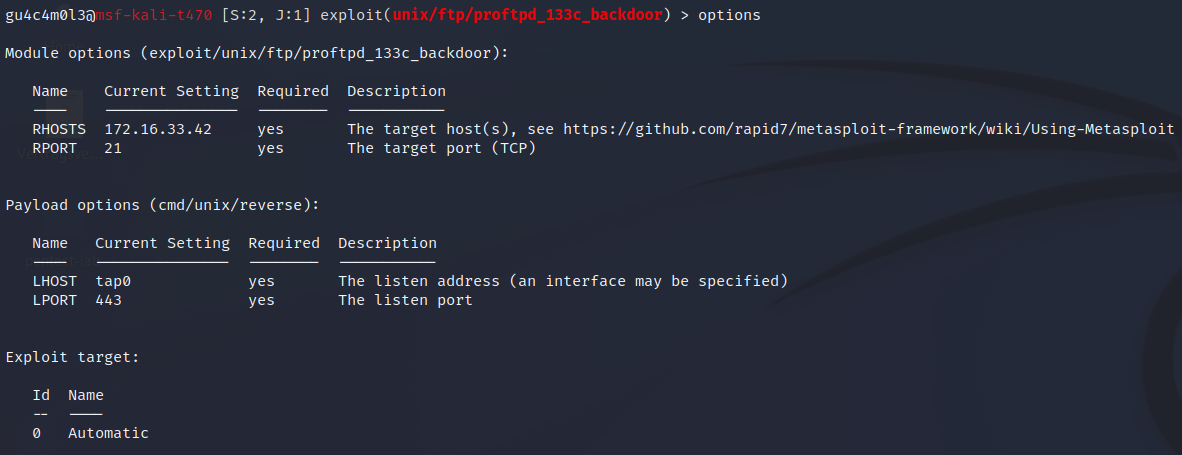
\includegraphics[width=\textwidth]{./img/vuln7_proftp/proftpd_exploit_config}
    \caption{Konfiguration des Metasploit-Moduls \texttt{exploit/unix/ftp/proftpd\_133c\_backdoor}}
    \label{fig:vuln7_metasploit_config}
\end{figure}

Abbildung \ref{fig:vuln7_metasploit_execution} zeigt die anschließende Ausführung des Exploits und den Erhalt der Root-Berechtigungen in Form einer Reverse-Shell.

\begin{figure}[h]
    \centering
    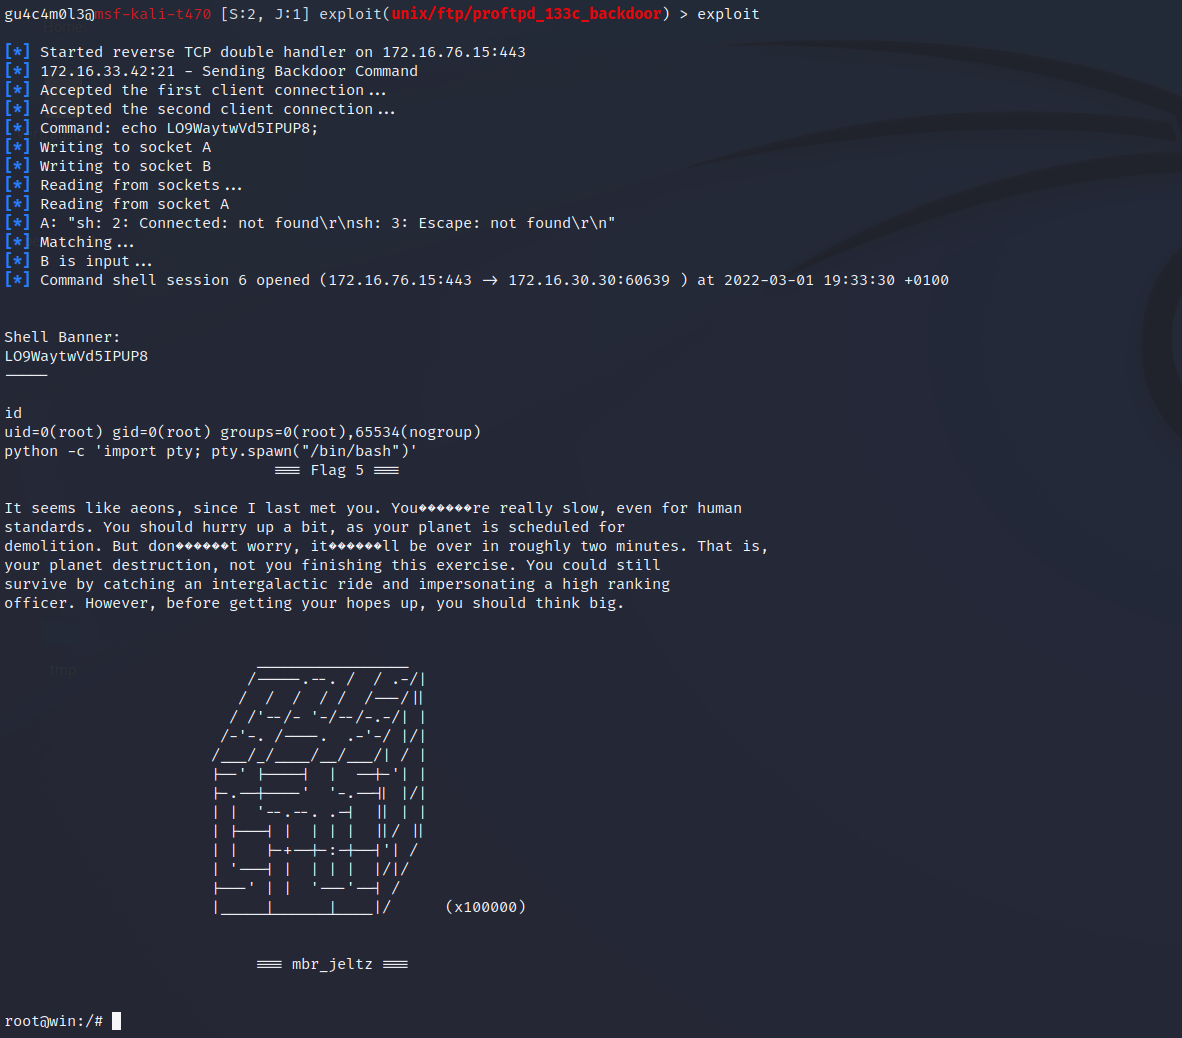
\includegraphics[width=\textwidth]{./img/vuln7_proftp/proftpd_exploit_run}
    \caption{Ausführung des Metasploit-Moduls \texttt{exploit/unix/ftp/proftpd\_133c\_backdoor}}
    \label{fig:vuln7_metasploit_execution}
\end{figure}


\subsection{Risikobewertung}
Aufgrund der Tatsache, dass mit der Schwachstelle 1 und der soeben behandelten Schwachstelle die externe Firewall und die DMZ-Firewall umgangen werden kann und Root-Berechtigungen über eine in der Öffentlichkeit seit 2010 bekannte Schwachstelle erlangt werden können, wird sowohl die Eintrittswahrscheinlichkeit als auch die Schadenshöhe mit HOCH bewertet.

Das Gesamtrisiko wurde daher mit \textcolor{red}{HOCH} bewertet.

\subsection{Empfohlene Gegenmaßnahmen}
Es wird empfohlen die neueste Version des ProFTPD-Servers zu installieren und die Version mit der Backdoor vom Server zu entfernen. 

\subsection{Hinterlassene Spuren und Spurenbeseitigung}
Nach der Durchführung des Penetration-Tests wurde die Reverse-Shell geschlossen.
